\documentclass[a4paper,class=article,border=10pt,tikz]{standalone}
\usepackage{tikz}
\usetikzlibrary{snakes,calc,positioning,patterns,angles,quotes,decorations.pathmorphing,decorations.markings,through}
\usetikzlibrary{arrows,decorations,decorations.text}
\usepackage{rotating}
\usetikzlibrary{arrows,decorations,decorations.text}
\usetikzlibrary{patterns.meta,math}




\usepackage{siunitx}

\begin{document}


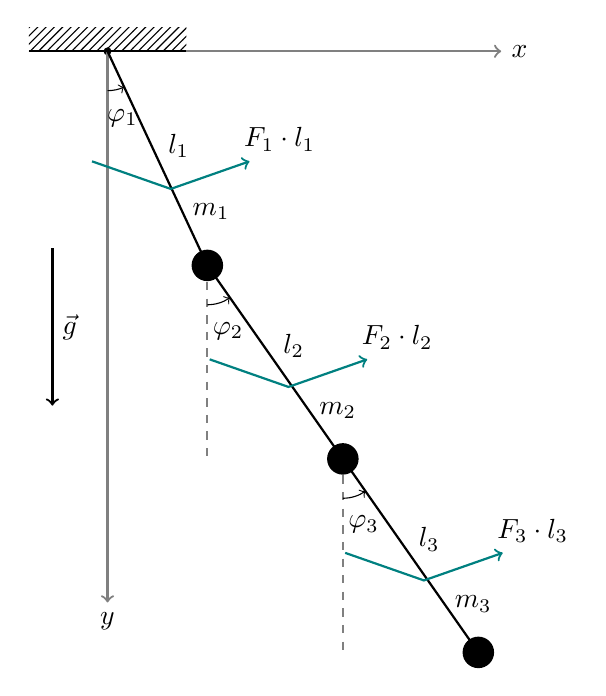
\begin{tikzpicture}
 \coordinate (origo) at (0,0);
 \coordinate (pivot) at (1,5);

    % draw axes
    \fill[black] (origo) circle (0.05);
    \draw[thick,gray,->] (origo) -- ++(5,0) node[black,right] {$x$};
    \draw[thick,gray,->] (origo) -- ++(0,-7) node (mary) [black,below] {$y$};
    \draw[thick,->] (-0.7,-2.5) -- (-0.7,-4.5) node[midway, right] {$\vec{g}$};

    % draw roof
    \fill[pattern = north east lines] ($ (origo) + (-1,0) $) rectangle ($ (origo) + (1,0.3) $);
    \draw[thick] ($ (origo) + (-1,0) $) -- ($ (origo) + (1,0) $);

    \draw[thick] (origo)  -- ++(295:3) coordinate (bob1) node[near end, right]{$m_{1}$};
    \node (l1_label) at ($(origo)+(307:1.5cm)$)   {$l_{1}$};
    \draw[thick,gray,dashed] (bob1) -- ++(0,-2.5) coordinate (line1);
    \fill (bob1) circle (0.2);
    \draw[thick] (bob1)  -- ++(305:3) coordinate (bob2) node[near end, right]{$m_{2}$};
    \node (l2_label) at ($(bob1)+(317:1.5cm)$)   {$l_{2}$};
    \draw[thick,gray,dashed] (bob2) -- ++(0,-2.5) coordinate (line2);
    \fill (bob2) circle (0.2);
    \draw[thick] (bob2)  -- ++(305:3) coordinate (bob3) node[near end, right]{$m_{3}$};
    \node (l3_label) at ($(bob2)+(317:1.5cm)$)   {$l_{3}$};
    \fill (bob3) circle (0.2);

    \pic [draw, ->, "$\varphi_1$", angle eccentricity=1.75] {angle = mary--origo--bob1};
    \pic [draw, ->, "$\varphi_2$", angle eccentricity=1.75] {angle = line1--bob1--bob2};
    \pic [draw, ->, "$\varphi_3$", angle eccentricity=1.75] {angle = line2--bob2--bob3};
    
    \draw[thick, teal,->] ($(origo)+(307:1.75cm)$) ++(-1.25cm,0cm)  --++(1cm,-0.35cm) --++ (1cm,0.35cm) node[above right,xshift=-0.2cm, black] {$F_1 \cdot l_1$};

    \draw[thick, teal,->] ($(bob1)+(317:1.75cm)$) ++(-1.25cm,0cm)  --++(1cm,-0.35cm) --++ (1cm,0.35cm) node[above right,xshift=-0.2cm, black] {$F_2 \cdot l_2$};


    \draw[thick, teal,->] ($(bob2)+(317:1.75cm)$) ++(-1.25cm,0cm)  --++(1cm,-0.35cm) --++ (1cm,0.35cm) node[above right,xshift=-0.2cm, black] {$F_3 \cdot l_3$};
\end{tikzpicture}


\end{document}
